%%%%%%%%%%%%%%%%%%%%%%%%%%%%%%%%%%%%%%%%%%%%%%%%%%%%%%%%%%%%%%%
%
% Welcome to writeLaTeX --- just edit your LaTeX on the left,
% and we'll compile it for you on the right. If you give
% someone the link to this page, they can edit at the same
% time. See the help menu above for more info. Enjoy!
%
%%%%%%%%%%%%%%%%%%%%%%%%%%%%%%%%%%%%%%%%%%%%%%%%%%%%%%%%%%%%%%%

% --------------------------------------------------------------
% This is all preamble stuff that you don't have to worry about.
% Head down to where it says "Start here"
% --------------------------------------------------------------
 
\documentclass[12pt]{article}
 
\usepackage[margin=1in]{geometry}
\usepackage{amsmath,amsthm,amssymb}
\usepackage{enumitem}
\usepackage{cancel}

\setlist[enumerate,1]{label={(\alph*)}} %this changes enumerate to (a),(b),...

\usepackage{graphicx} %package to manage images

\newcommand{\A}{{\mathcal{A}}}
\newcommand{\C}{{\mathbb C}}
\newcommand{\CC}{{\mathcal{C}}}
\newcommand{\N}{{\mathbb N}}
\newcommand{\R}{{\mathbb R}}
\newcommand{\Q}{{\mathbb Q}}
\newcommand{\Z}{{\mathbb Z}}

\newcommand{\Aut}{{\rm Aut}}
\newcommand{\End}{{\rm End}}
\newcommand{\Hom}{{\rm Hom}}
\newcommand{\id}{{\rm id}}
\newcommand{\Ima}{{\rm Im}}
\newcommand{\Ker}{{\rm Ker}}
\newcommand{\Mor}{{\rm Mor}}
\newcommand{\Rad}{{\rm Rad}}
\newcommand{\Prob}{{\rm P}}

\renewcommand\labelitemi{-} %this changes itemize bullet points to dashes (-)

\usepackage{listings}
\usepackage{xcolor}

%New colors defined below
\definecolor{codegreen}{rgb}{0,0.6,0}
\definecolor{codegray}{rgb}{0.5,0.5,0.5}
\definecolor{codepurple}{rgb}{0.58,0,0.82}
\definecolor{backcolour}{rgb}{0.95,0.95,0.92}

%Code listing style named "mystyle"
\lstdefinestyle{mystyle}{
  backgroundcolor=\color{backcolour}, commentstyle=\color{codegreen},
  keywordstyle=\color{magenta},
  numberstyle=\tiny\color{codegray},
  stringstyle=\color{codepurple},
  basicstyle=\ttfamily\footnotesize,
  breakatwhitespace=false,         
  breaklines=true,                 
  captionpos=b,                    
  keepspaces=true,                 
  numbers=left,                    
  numbersep=5pt,                  
  showspaces=false,                
  showstringspaces=false,
  showtabs=false,                  
  tabsize=2
}

%"mystyle" code listing set
\lstset{style=mystyle}
 
\newenvironment{theorem}[2][Theorem]{\begin{trivlist}
\item[\hskip \labelsep {\bfseries #1}\hskip \labelsep {\bfseries #2.}]}
{\end{trivlist}}
\newenvironment{lemma}[2][Lemma]{\begin{trivlist}
\item[\hskip \labelsep {\bfseries #1}\hskip \labelsep {\bfseries #2.}]}
{\end{trivlist}}
\newenvironment{exercise}[2][Exercise]{\begin{trivlist}
\item[\hskip \labelsep {\bfseries #1}\hskip \labelsep {\bfseries #2.}]}
{\end{trivlist}}
\newenvironment{problem}[2][Problem]{\begin{trivlist}
\item[\hskip \labelsep {\bfseries #1}\hskip \labelsep {\bfseries #2.}]}
{\end{trivlist}}
\newenvironment{question}[2][Question]{\begin{trivlist}
\item[\hskip \labelsep {\bfseries #1}\hskip \labelsep {\bfseries #2.}]}
{\end{trivlist}}
\newenvironment{corollary}[2][Corollary]{\begin{trivlist}
\item[\hskip \labelsep {\bfseries #1}\hskip \labelsep {\bfseries #2.}]}
{\end{trivlist}}

\newenvironment{solution}{\begin{proof}[Solution]}{\end{proof}}
 
\begin{document}
 
% --------------------------------------------------------------
%                         Start here
% --------------------------------------------------------------
 
\title{Homework 3}%replace X with the appropriate number
\author{Mengxiang Jiang\\ %replace with your name
Stat 610 Distribution Theory} %if necessary, replace with your course title
 
\maketitle
 
\begin{problem}{1} %You can use theorem, exercise, problem, or question here.
  \textit{Statistical Inference} by Casella and Berger, 2nd Edition, Chapter 1, 
  Exercise 47 parts b and c.
  \begin{itemize}
    \item[47.] Prove the following functions are cdfs.
    \begin{itemize}
      \item [(b)] $\left(1 + e^{-x}\right)^{-1},\;x \in (-\infty, \infty)$
      \item [(c)] $e^{-e^{-x}},\; x \in (-\infty, \infty)$
    \end{itemize}

    \begin{theorem}{2.6} $F(x)$ is a cdf for some rv $X$ if and only if
      \begin{itemize}
        \item[i.] $x \le y \Rightarrow F(x) \le F(y)$ (nondecreasing)
        \item[ii.] $F(y) \rightarrow F(x)$ as $y \downarrow x$ (right-continuous)
        \item[iii.] $F(x) \rightarrow 0$ as $x \rightarrow -\infty$
        and $F(x) \rightarrow 1$ as $x \rightarrow \infty$ (total measure 1) 
      \end{itemize}
      
    \end{theorem}

    \begin{itemize}
      \item [(b)]
      \begin{itemize}
        \item[i.] $F'(x) = \frac{e^{-x}}{(1+e^{-x})^2}$, which is nonnegative
        for all x, so $F$ is nondecreasing.
        \item[ii.] Since $F$ is differentiable everywhere, 
        it is continuous everywhere, so it is also right continuous.
        \item[iii.] 
        \[
          \lim_{x \to -\infty} \frac{1}{1+e^{-x}} = \frac{1}{\infty} = 0.
        \]
        \[
          \lim_{x \to \infty} \frac{1}{1+e^{-x}} = \frac{1}{1} = 1.
        \]
      \end{itemize}
      \item [(c)]
      \begin{itemize}
        \item[i.] $F'(x) = e^{-x}e^{-e^{-x}}$, which is nonnegative for all x,
        so $F$ is nondecreasing.
        \item[ii.] Since $F$ is differentiable everywhere, 
        it is continuous everywhere, so it is also right continuous.
        \item[iii.] 
        \[
          \lim_{x \to -\infty} e^{-e^{-x}} = e^{-e^{\infty}} = e^{-\infty} = 0.
        \]
        \[
          \lim_{x \to \infty} e^{-e^{-x}} = e^{-e^{-\infty}} = e^{0} = 1.
        \]
      \end{itemize}
    \end{itemize}
  \end{itemize}
\end{problem}

\begin{problem}{2}
  Suppose we sample 10 individuals at random and with replacement from a 
  population that has three categories $C_1, C_2, C_3$ with respective 
  proportions $10\%$, $30\%$ and $60\%$. Let $X_i$ be the number in the 
  sample from $C_i$, $i = 1, 2, 3$. Then (recall Example 1.11 on Slide 
  31 in the notes)
  \[
    \Prob(X_1 = i, X_2 = j \text{ and } X_3 = k) = 
    \frac{10!}{i!j!k!}0.1^i0.3^j0.6^k, \quad
    \text{if } i+j+k=10,\; i \ge 0,\;j \ge 0,\; k \ge 0.
  \]
  \begin{enumerate}
    \item Determine the probability that $X_1$ and $X_2$ are both equal 1 
    (keeping in mind what $X_3$ must be).
    \item Find the probability that $X_1 = X_2$ by splitting the event into 
    disjoint cases according to their common value, and then get the 
    conditional probability that $X_1 = X_2 = 1$, given $X_1 = X_2$. 
    (Recall Problem 2(b) of Assignment 2.)
    \item Call $C_1$ ``Success" and $C_1^c$ ``Failure" to argue that 
    $X_1$ has binomial(10, 0.1) distribution. Draw a similar conclusion 
    about $X_2$.
    \item Are the events $\{X1 = 1\}$ and $\{X_2 = 1\}$ independent? Explain.
  \end{enumerate}
  \begin{enumerate}
    \item Since $i+j+k=10$, $X_3 = k = 10-i-j = 8$.
    \[
      \Prob(X_1=1,X_2=1,X_3=8) = 
      \frac{10!}{1!1!8!}(0.1)(0.3)(0.6^8) =
      90(0.1)(0.3)(0.6^8) \approx 0.0453.
    \]
    \item Let the common value be $t = X_1=X_2$, then $X_3 = 10-2t$.\\
    Since $X_3 \ge 0$, thus $t = 0,1,2,3,4,5$.
    \[
      \Prob(X_1=X_2=t, X_3=10-2t) =
      \sum_{t=0}^5 \frac{10!}{t!t!(10-2t)!}0.1^t0.3^t0.6^{10-2t}
      \approx 0.120.
    \]
    \[
      \Prob(X_1=X_2=1 \mid X_1=X_2) =
      \frac{\Prob(X_1=1,X_2=1)}{\Prob(X_1=X_2)} \approx
      \frac{0.0453}{0.120} \approx 0.378.
    \]
    \item Declare ``Success" = draw is in $C_1$ (prob $0.1$), 
    ``Failure" = not in $C_1$ (prob $0.9$). Across 10 independent draws
    \[
      \Prob(X_1 = k) = \binom{10}{k} 0.1^k 0.9^{10-k},\quad k=0,1,\ldots,10.
    \]
    So $X_1 \sim$ binomial(10, 0.1).\\
    Similarly, declare ``Success" = draw is in $C_2$ (prob $0.3$), 
    ``Failure" = not in $C_2$ (prob $0.7$). Across 10 independent draws
    \[
      \Prob(X_2 = k) = \binom{10}{k} 0.3^k 0.7^{10-k},\quad k=0,1,\ldots,10.
    \]
    So $X_2 \sim$ binomial(10, 0.3).
    \item
    \[
      \Prob(X_1=1) = \binom{10}{1}0.1^1 0.9^9 \approx 0.387.
    \]
    \[
      \Prob(X_2=1) = \binom{10}{1}0.3^1 0.7^9 \approx 0.121.
    \]
    \[
      \Prob(X_1=1)\Prob(X_2=1) \approx 0.387 \times 0.121 \approx 0.047.
    \]
    \[
      \Prob(X_1=1,X_2=1) \approx 0.0453 \ne
      \Prob(X_1=1)\Prob(X_2=1) \approx 0.047.
    \]
    So the events $\{X_1=1\}$ and $\{X_2=1\}$ are not independent.
  \end{enumerate}
\end{problem}

\begin{problem}{3}
  Determine whether the following functions are cdfs or not, 
  explaining your reasoning. If it is a cdf, is it discrete, continuous 
  or a mixture of the two? You may assume the interval given for the variable 
  is the ostensible support (no probability outside that interval). 
  It may help to plot the functions.
  \begin{enumerate}
    \item $F(t) = t(2-t)$ for $t \in [0,1]$.
    \item $F(t) = t(2-t)$ for $t \in [0,2]$.
    \item $F(t) = t(2-t)1_{[0,1/2)}(t) + \frac{t+7}{8}1_{[1/2,1]}(t)$ 
    for $t \in [0,1]$.
    \item $F(t) = \frac15 1_{[0,\infty)}(t) + \frac14 1_{[1/2,\infty)}(t)
    + \frac12 1_{[3/4,\infty)}(t) + \frac{1}{20} 1_{[1,\infty)}(t)$
    for $t \in [0,1]$.
  \end{enumerate}
  \pagebreak
  \begin{enumerate}
    \item graph of $F$:
    \begin{center}
      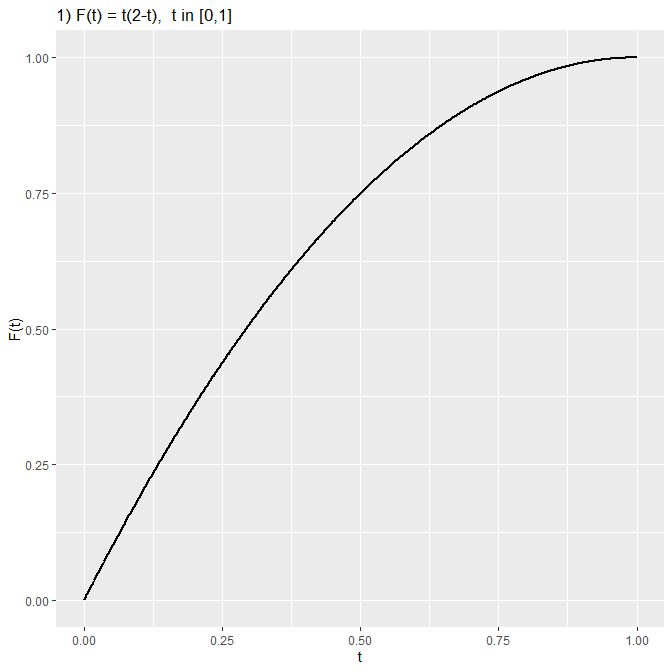
\includegraphics[width=0.8\textwidth]{3a.png}
    \end{center}
    Assuming $F(t) = 0$ for $t < 0$ and $t > 1$, 
    then $F$ fails both right-continuity and total measure 1.
    So $F$ is not a cdf. However, if we assume $F(t) = 0$ for $t < 0$
    and $F(t) = 1$ for $t > 1$, then $F$ is a cdf, which is continuous.
    \pagebreak
    \item graph of $F$:
    \begin{center}
      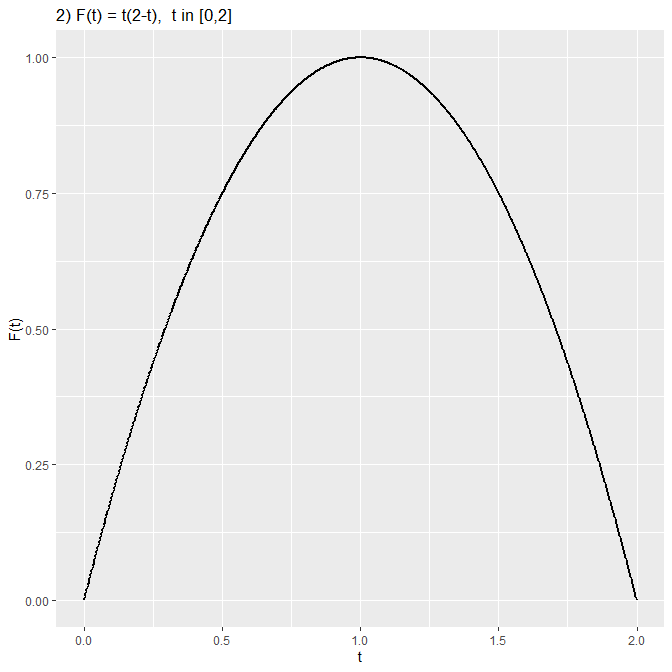
\includegraphics[width=0.8\textwidth]{3b.png}
    \end{center}
    $F$ fails nondecreasing, since $F'(t) = 2-2t < 0$ for $t > 1$,
    so $F$ is not a cdf.
    \pagebreak
    \item graph of $F$:
    \begin{center}
      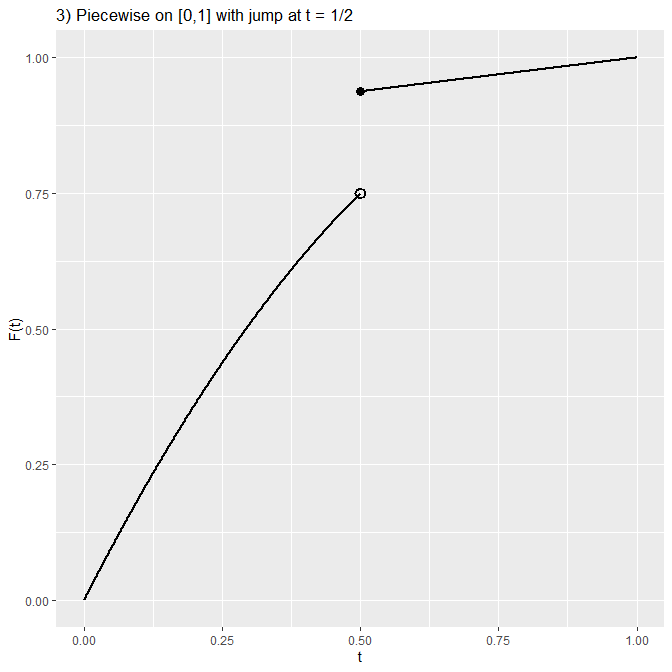
\includegraphics[width=0.8\textwidth]{3c.png}
    \end{center}
    Assuming $F(t) = 0$ for $t < 0$ and $t > 1$, 
    then $F$ fails both right-continuity and total measure 1.
    So $F$ is not a cdf. However, if we assume $F(t) = 0$ for $t < 0$
    and $F(t) = 1$ for $t > 1$, then $F$ is a cdf, which is a mixture of
    continuous and discrete.
    \pagebreak
    \item graph of $F$:
    \begin{center}
      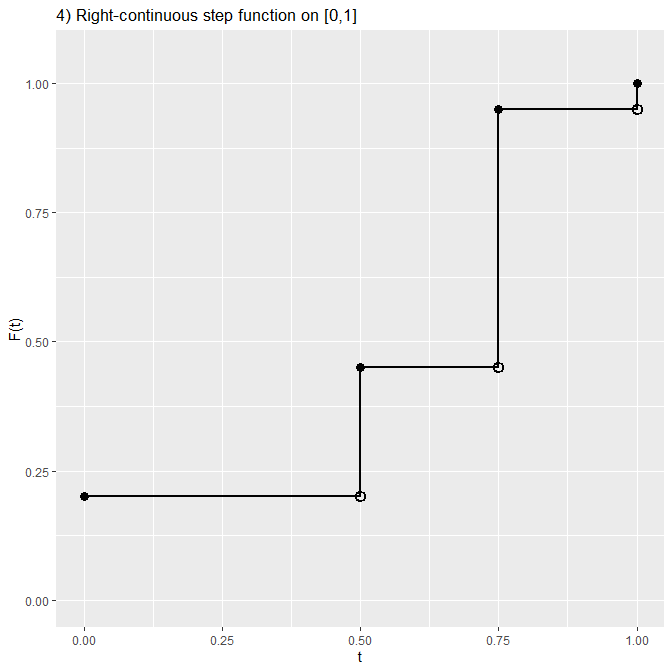
\includegraphics[width=0.8\textwidth]{3d.png}
    \end{center}
    $F$ satisfies all three properties of a cdf, so $F$ is a cdf,
    which is discrete.
  \end{enumerate}
\end{problem}

\begin{problem}{4}
  Let $U$ have uniform(0,1) distribution (see Example 2.6 in the notes). 
  Let $V = \sqrt{U}$. Show that $V$ is a continuous random variable 
  and find its cdf. Find the pdf and plot both the cdf and the pdf.
  \\\\
  Since $U$ is continuous, and $V = \sqrt{U}$ is a continuous function,
  so $V$ is also continuous. Because $g(u) = \sqrt{u}$ is nondecreasing,
  we can get the cdf of $V$ by inverting $g$:
  \[
    g^{-1}(v) = v^2, \quad v \in [0,1].
  \]
  For $v \in [0,1]$,
  \[
    F_V(v) = \Prob(V \le v) = \Prob(\sqrt{U} \le v) = \Prob(U \le v^2) = F_U(v^2).
  \]
  However, it must be noted that $F_U(u) = 0$ for $u < 0$ and
  $F_U(u) = 1$ for $u > 1$. So the cdf of $V$ is
  \[
    F_V(v) = v^2 1_{[0,1]}(v) + 0 \cdot 1_{(-\infty,0)}(v) 
    + 1 \cdot 1_{(1,\infty)}(v).
  \]
  The pdf of $V$ is
  \[
    f_V(v) = F_V'(v) = 2v 1_{[0,1]}(v).
  \]
  The graphs of the pdf and cdf of $V$ are shown below.
  \begin{center}
    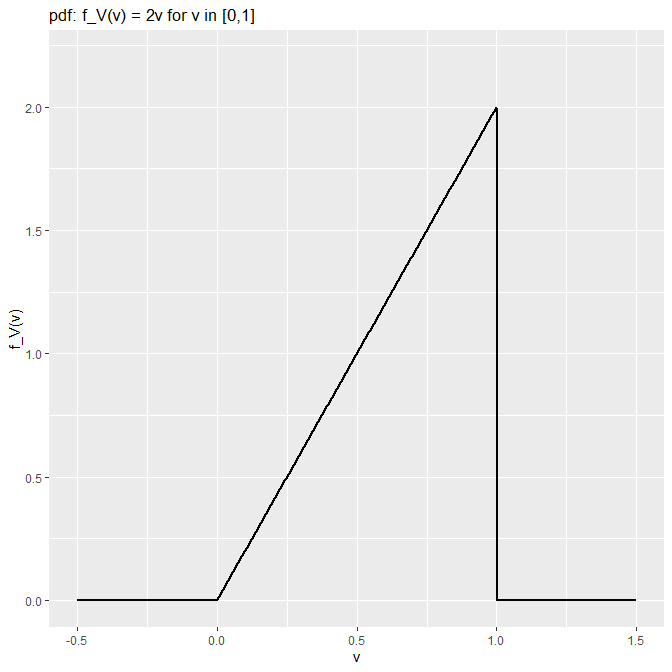
\includegraphics[width=0.6\textwidth]{4pdf.png}
    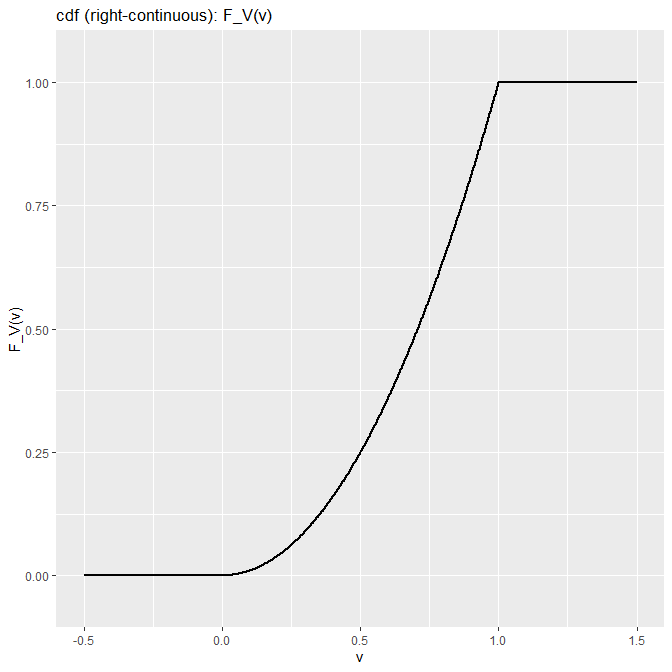
\includegraphics[width=0.6\textwidth]{4cdf.png}
  \end{center}
\end{problem}

\pagebreak

\begin{problem}{5}
  Suppose $T_1$ and $T_2$ are two random variables such that 
  $T_1(s) \le T_2(s)$ for all outcomes $s$ in the sample space. 
  Prove that $F_{T_1}(t) \ge F_{T_2}(t)$ for all real $t$. 
  Hint: compare appropriate events about the random variables.
  \\\\
  For any real $t$, let $A = \{s: T_1(s) \le t\}$ and $B = \{s: T_2(s) \le t\}$.
  If $s \in B$, then $T_2(s) \le t$. Since $T_1(s) \le T_2(s)$,
  so $T_1(s) \le t$ implies $s \in A$. Thus $B \subseteq A$. 
  Thus $\Prob(A) \ge \Prob(B)$, i.e.
  \[
    F_{T_1}(t) = \Prob(T_1 \le t) \ge \Prob(T_2 \le t) = F_{T_2}(t).
  \]
\end{problem}

\begin{problem}{6}
  \textit{Statistical Inference} by Casella and Berger, 2nd Edition, Chapter 2, 
  Exercise 1 parts a and b.
  \begin{itemize}
    \item [1.] In each of the following, find the pdf of $Y$. Show that
    the pdf integrates to 1.
    \begin{enumerate}
      \item $Y = X^3$ and $f_X(x) = 42x^5(1-x),\;0 < x < 1$.
      \item $Y = 4X+3$ and $f_X(x) = 7e^{-7x},\;0 < x < \infty$.
    \end{enumerate}
    \begin{enumerate}
      \item $Y = X^3 \Rightarrow X = Y^{1/3}$, and
      \[
        \frac{dX}{dY} = \frac{1}{3}Y^{-2/3}.
      \]
      The support of $Y$ is $(0,1)$.
      \[
        f_Y(y) = f_X(y^{1/3}) \left|\frac{dX}{dY}\right| =
        42(y^{1/3})^5(1-y^{1/3}) \cdot \frac{1}{3}y^{-2/3} =
        14y(1-y^{1/3}),\quad 0 < y < 1.
      \]
      \[
      \begin{aligned}
        \int_0^1 14y(1-y^{1/3}) dy &= \int_0^1 14(y - y^{4/3}) dy \\
        &=\left[7y^2 - \frac{14}{\frac{4}{3}+1}y^{\frac{4}{3}+1}\right]_0^1 \\
        &=7 - \frac{14}{\frac{4}{3}+1} = 7 - 6 = 1.
      \end{aligned}
      \]
      \item $Y = 4X+3 \Rightarrow X = \frac{Y-3}{4}$, and
      \[
        \frac{dX}{dY} = \frac{1}{4}.
      \]
      The support of $Y$ is $(3,\infty)$.
      \[
        f_Y(y) = f_X\left(\frac{y-3}{4}\right) \left|\frac{dX}{dY}\right| =
        7e^{-7\frac{y-3}{4}} \cdot \frac{1}{4} =
        \frac{7}{4}e^{-\frac{7}{4}(y-3)},\quad y > 3.
      \]
      \[
        \int_3^\infty \frac{7}{4}e^{-\frac{7}{4}(y-3)} dy =
        \left[-e^{-\frac{7}{4}(y-3)}\right]_3^\infty = 0 - (-1) = 1.
      \]
    \end{enumerate}
  \end{itemize}
\end{problem}

\begin{problem}{7}
  Let $X$ be a continuous random variable, 
  \textit{not necessarily nonnegative,}
  with cdf $F_X$ and pdf $f_X$.
  \begin{enumerate}
    \item Find the cdf for $Y = |X|$ and use it to find the pdf for $Y$. 
    Be sure that both satisfy the necessary properties.
    \item Apply the above to the standard normal density 
    $f_X (x) = \frac{1}{\sqrt{2\pi}} e^{-\frac{x^2}{2}}$. 
    (This gives the so-called half-normal pdf.)
  \end{enumerate}
  \begin{enumerate}
    \item For $y < 0$, $F_Y(y) = \Prob(Y \le y) = 0$.\\
    For $y \ge 0$, $F_Y(y) = \Prob(Y \le y) = \Prob(|X| \le y) 
    = \Prob(-y \le X \le y) = F_X(y) - F_X(-y)$.
    Thus, the pdf of $Y$ is
    \[
      f_Y(y) = F_Y'(y) = f_X(y) + f_X(-y), \quad y \ge 0.
    \]
    $f_Y(y) \ge 0$ for all $y$ since $f_X$ is nonnegative and
    \[
    \begin{aligned}
      \int_{-\infty}^\infty f_Y(y) dy &= \int_0^\infty (f_X(y) + f_X(-y)) dy \\
      &= \int_0^\infty f_X(y) dy + \int_{-\infty}^0 f_X(y) dy \\
      &= \int_{-\infty}^\infty f_X(y) dy = 1.
    \end{aligned}
    \]
    \item Plugging in the pdf of $X$ gives
    \[
      f_Y(y) = F_Y'(y) = f_X(y) + f_X(-y) =
      \frac{1}{\sqrt{2\pi}} e^{-\frac{y^2}{2}} +
      \frac{1}{\sqrt{2\pi}} e^{-\frac{(-y)^2}{2}} =
      \frac{2}{\sqrt{2\pi}} e^{-\frac{y^2}{2}}, \quad y \ge 0.
    \]
    $f_Y(y) \ge 0$ for all $y$ and
    \[
    \begin{aligned}
      \int_{-\infty}^\infty f_Y(y) dy 
      &= \int_0^\infty \frac{2}{\sqrt{2\pi}} e^{-\frac{y^2}{2}} dy \\
      &= 2 \int_0^\infty \frac{1}{\sqrt{2\pi}} e^{-\frac{y^2}{2}} dy \\
      &= 2 \cdot \frac{1}{2} = 1.
    \end{aligned}
    \]
  \end{enumerate}
\end{problem}

\begin{problem}{8}
  Let $h(x) = xe^{-2x}$ for $x > 0$, and $h(x) = 0$ otherwise.
  \begin{enumerate}
    \item Find $c > 0$ such that $f (x) = ch(x)$ is a valid pdf.
    \item Find the corresponding cdf. (Check that it satisfies the 
    required properties of a cdf.)
    \item Plot both the pdf and the cdf.
    \item Suppose $X$ has pdf $f (x)$. Find the cdf and pdf for 
    $Y = \log(X)$. (This is the natural logarithm.)
  \end{enumerate}

  \begin{enumerate}
    \item To make $f(x) = ch(x)$ a valid pdf, we need
    \[
      \int_{-\infty}^\infty f(x) dx = 1 \implies c \int_0^\infty h(x) dx = 1.
    \]
    First, we compute the integral:
    \[
      \int_0^\infty h(x) dx = \int_0^\infty xe^{-2x} dx.
    \]
    Using integration by parts with $u = x$ and $dv = e^{-2x} dx$, 
    we have $du = dx$ and $v = -\frac{1}{2} e^{-2x}$. Thus,
    \[
      \int_0^\infty xe^{-2x} dx 
      = \left[-\frac{1}{2}xe^{-2x}\right]_0^\infty 
      + \frac{1}{2}\int_0^\infty e^{-2x} dx.
    \]
    The first term evaluates to $0$ by L'Hôpital's rule 
    \[
      \lim_{x \to \infty} -\frac{x}{2e^{2x}} 
      = \lim_{x \to \infty} -\frac{1}{4e^{2x}} = 0. 
    \]
    and the second term is
    \[
      \frac{1}{2}\int_0^\infty e^{-2x} dx
      = \frac{1}{2}\left[-\frac{1}{2}e^{-2x}\right]_0^\infty
      = \frac{1}{2} \cdot \frac{1}{2} = \frac{1}{4}.
    \]
    Therefore,
    \[
      \int_0^\infty h(x) dx 
      = \frac{1}{4} \implies c \cdot \frac{1}{4} = 1 \implies c = 4.
    \]
    So the valid pdf is
    \[
      f(x) = 4xe^{-2x}, \quad x > 0.
    \]
    \item The corresponding cdf is
    \[
      F(x) = \int_{-\infty}^x f(t) dt = \int_0^x 4h(t) dt = 4\int_0^x te^{-2t} dt.
    \]
    Using integration by parts again with $u = t$ and $dv = e^{-2t} dt$, we find
    \[
      \int_0^x te^{-2t} dt = \left[-\frac{1}{2}te^{-2t}\right]_0^x + \frac{1}{2}\int_0^x e^{-2t} dt.
    \]
    The first term evaluates to $-\frac{1}{2}xe^{-2x}$, and the second term is
    \[
      \frac{1}{2}\int_0^x e^{-2t} dt = \frac{1}{2}\left[-\frac{1}{2}e^{-2t}\right]_0^x = \frac{1}{4}(1 - e^{-2x}).
    \]
    Therefore,
    \[
      \int_0^x te^{-2t} dt = -\frac{1}{2}xe^{-2x} + \frac{1}{4}(1 - e^{-2x}),
    \]
    and
    \[
      F(x) = 4\left(-\frac{1}{2}xe^{-2x} + \frac{1}{4}(1 - e^{-2x})\right) = -2xe^{-2x} + (1 - e^{-2x}).
    \]
    Thus,
    \[
      F(x) = 1 - e^{-2x} - 2xe^{-2x}, \quad x > 0.
    \]
    For $x \le 0$, $F(x) = 0$.\\
    We check the properties of a cdf:
    \begin{itemize}
      \item[i.] $F(x)$ is nondecreasing since $F'(x) = f(x) = 4xe^{-2x} \ge 0$ for $x > 0$.
      \item[ii.] $F(x)$ is right-continuous since it is differentiable everywhere.
      \item[iii.] 
      \[
        \lim_{x \to -\infty} F(x) = 0, \text{ since } F(x) = 0 \text{ for } x \le 0.
      \]
      \[
        \lim_{x \to \infty} F(x) 
        = \lim_{x \to \infty} (1 - e^{-2x} - 2xe^{-2x}) 
        = 1 - 0 - \infty \cdot 0 \text{(indeterminate form)}.
      \]
      Using L'Hôpital's rule on $2xe^{-2x}$:
      \[
        \lim_{x \to \infty} 2xe^{-2x} 
        = \lim_{x \to \infty} \frac{2x}{e^{2x}} 
        = \lim_{x \to \infty} \frac{2}{2e^{2x}} = 0.
      \]
      Thus,
      \[
        \lim_{x \to \infty} F(x) = 1 - 0 - 0 = 1.
      \]
    \end{itemize}
    \item The graphs of the pdf and cdf are shown below.
    \begin{center}
      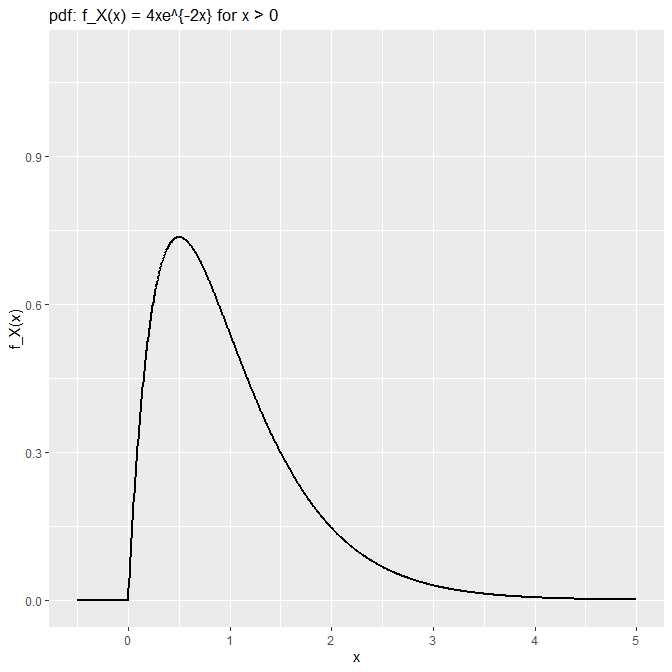
\includegraphics[width=0.6\textwidth]{8pdf.png}
      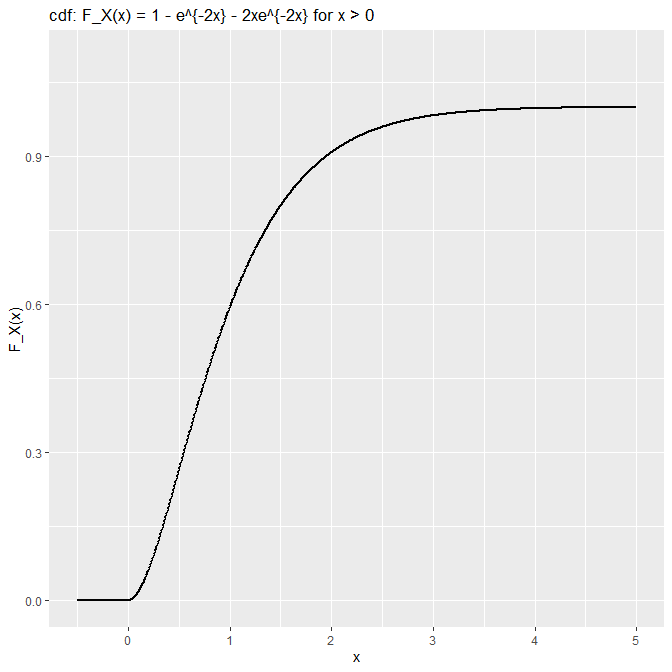
\includegraphics[width=0.6\textwidth]{8cdf.png}
    \end{center}
    \item Since $Y = \log(X) \Rightarrow X = e^Y$, and
    \[
      \frac{dX}{dY} = e^Y.
    \]
    The support of $Y$ is $(-\infty, \infty)$.
    \[
      f_Y(y) = f_X(e^y) \left|\frac{dX}{dY}\right| =
      4(e^y)e^{-2(e^y)} \cdot e^y =
      4e^{2y}e^{-2e^y},\quad y \in (-\infty, \infty).
    \]
    This is a valid pdf since $f_Y(y) \ge 0$ for all $y$ and
    \[
    \begin{aligned}
      \int_{-\infty}^\infty f_Y(y) dy 
      &= \int_{-\infty}^\infty 4e^{2y}e^{-2e^y} dy \\
      &= \int_0^\infty 4u e^{-2u} du \text{ (using substitution } u = e^y) \\
      &= 1 \text{ (as computed in part (a)).}
    \end{aligned}
    \]
    The cdf of $Y$ is
    \[
      F_Y(y) = \int_{-\infty}^y f_Y(t) dt = \int_{-\infty}^y 4e^{2t}e^{-2e^t} dt.
    \]
    Using substitution $u = e^t$, $du = e^t dt$, we have
    \[
      F_Y(y) = \int_0^{e^y} 4u e^{-2u} du.
    \]
    Using integration by parts with $v = u$ and $dw = e^{-2u} du$, we find
    \[
    \begin{aligned}
      \int_0^{e^y} 4u e^{-2u} du 
      &= 4\left[-\frac{1}{2}ue^{-2u}\right]_0^{e^y} 
      + 4\cdot\frac{1}{2}\int_0^{e^y} e^{-2u} du \\
      &= -2e^y e^{-2e^y} + 2\int_0^{e^y} e^{-2u} du \\
      &= -2e^y e^{-2e^y} + 2\left[-\frac{1}{2}e^{-2u}\right]_0^{e^y} \\
      &= -2e^y e^{-2e^y} + (1 - e^{-2e^y}).
    \end{aligned}
    \]
    We check the properties of a cdf:
    \begin{itemize}
      \item[i.] $F_Y(y)$ is nondecreasing since $F_Y'(y) = f_Y(y) = 4e^{2y}e^{-2e^y} \ge 0$ for all $y$.
      \item[ii.] $F_Y(y)$ is right-continuous since it is differentiable everywhere.
      \item[iii.] 
      \[
        \lim_{y \to -\infty} F_Y(y) = 0, \text{ since } e^y \to 0.
      \]
      \[
        \lim_{y \to \infty} F_Y(y) 
        = \lim_{y \to \infty} (1 - e^{-2e^y} - 2e^y e^{-2e^y}) 
        = 1 - 0 - \infty \cdot 0 \text{(indeterminate form)}.
      \]
      Using L'Hôpital's rule on $2e^y e^{-2e^y}$:
      \[
        \lim_{y \to \infty} 2e^y e^{-2e^y} 
        = \lim_{y \to \infty} \frac{2e^y}{e^{2e^y}} 
        = \lim_{y \to \infty} \frac{2e^y}{2e^y e^{2e^y}} 
        = \lim_{y \to \infty} e^{-2e^y} = 0.
      \]
      Thus,
      \[
        \lim_{y \to \infty} F_Y(y) = 1 - 0 - 0 = 1.
      \]
    \end{itemize}
  \end{enumerate}
\end{problem}

% --------------------------------------------------------------
%     You don't have to mess with anything below this line.
% --------------------------------------------------------------
\end{document}
